\smallframetitle

\section{Semaine du 14/05/24 au 21/05/24}
\insertsectionframe
\subsection{Le jeu de donnée}
\insertsubsectionframe

\begin{frame}{Le jeu de donnée}
    \begin{block}{Arcep}
        L'autorité de régulation des communications électroniques, des postes et de la distribution de la presse (Arcep) est une autorité administrative indépendante française chargée de réguler les communications électroniques et postales et la distribution de la presse.
    \end{block}

    \begin{block}{Mon Réseau Mobile}
        Mon Réseau Mobile est la plate-forme cartographique regroupant l’ensemble des données géographiques en lien avec les réseaux dits \og mobiles \fg{} (2G, 3G, 4G, 5G) régulés par l’Arcep.
    \end{block}

    \begin{alertblock}{Nouvelle mise à jour}
        Une nouvelle mise à jour des données est prévue de \textbf{jeudi 20 juin 2024} à 17h40 : données du 1\ier{} trimestre de 2024.
    \end{alertblock}

    A cette adresse : \url{https://www.data.gouv.fr/fr/datasets/mon-reseau-mobile/\#/discussions}, on peut poser nos questions sur le jeu de données.
\end{frame}


\begin{frame}{Arborescence du jeu de données}
    \begin{columns}
        \begin{column}{0.4\textwidth}
            Les fichiers de données sont rangés par trimestre de publication, zone (France métropolitaine/Outre-mer) et département le cas échéant :
        \end{column}
            
        \begin{column}{0.6\textwidth}
            \begin{figure}
                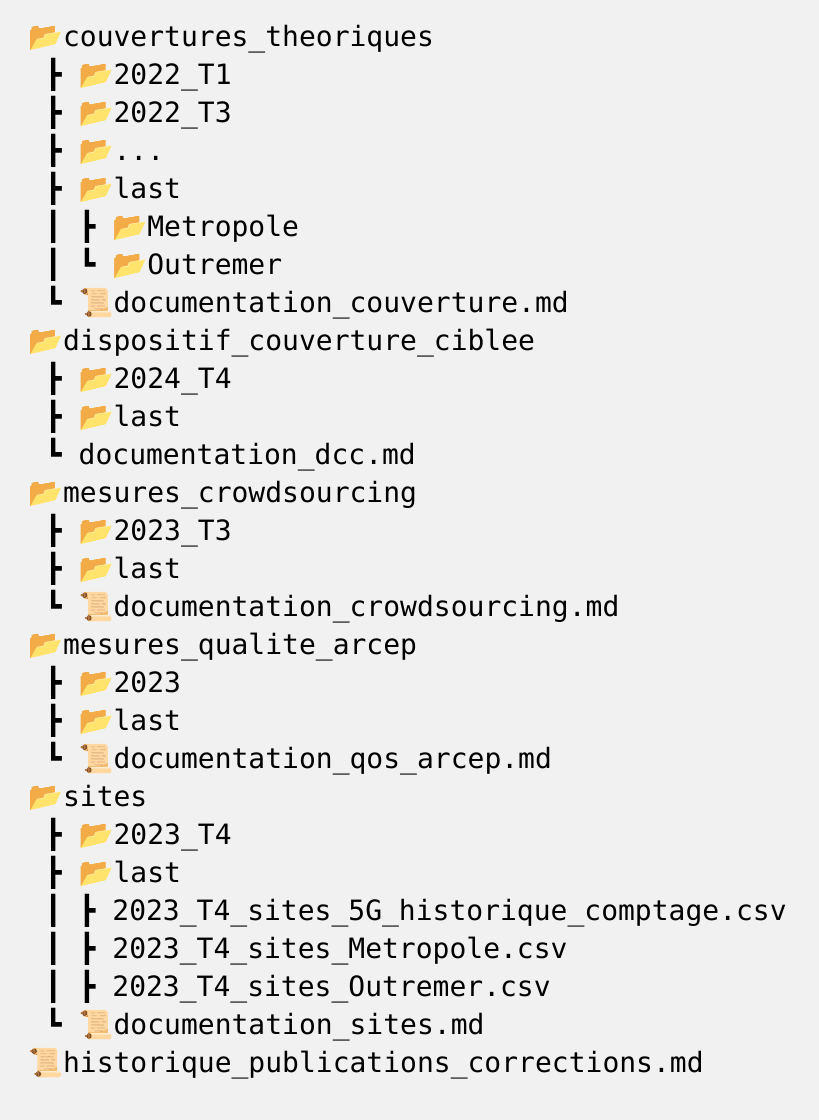
\includegraphics[height=0.55\paperheight]{images/architecture.png}
                \caption{\label{fig:archi}Architecture de la base de donnée}
            \end{figure}
        \end{column}
    \end{columns} 
    
\end{frame}

\begin{frame}{Fréquences de mises à jour}
    \begin{figure}
        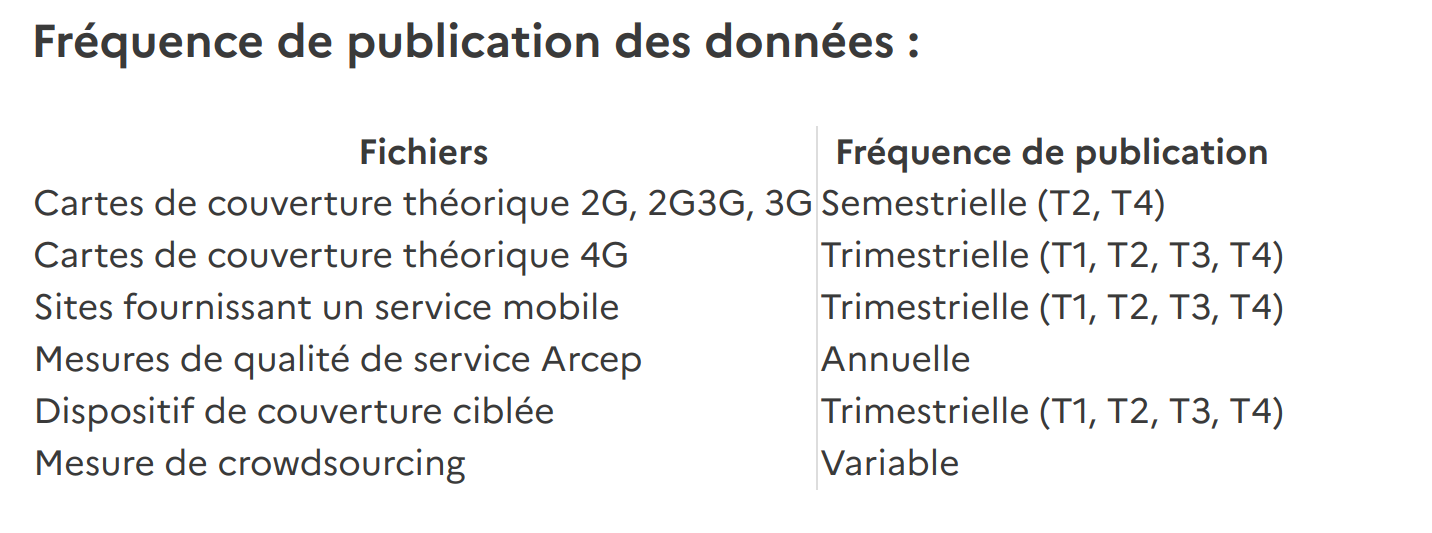
\includegraphics[height=0.5\paperheight]{images/frequence.png}
        \caption{\label{fig:freq}Fréquence de publication de mises à jour}
    \end{figure}
\end{frame}


\subsection{Faisons parler les données}
\insertsubsectionframe

\begin{frame}{Quelques chiffres en vrac}
    Tout d'abord, remarquons que chaque station peut être identifiée à son \texttt{num\_site} (seul deux stations n'en n'ont pas).
    Ensuite, voici ce que l'on a découvert :
    \begin{block}{Des chiffres sympathiques}
        \begin{itemize}
            \item \texttt{site\_zb} : $10\,596$ (Site issu du programme \og zones blanches – centres-bourgs\fg{}) ;
            \item \texttt{site\_dcc} : $10\,627$ (Site issu du \og Dispositif de Couverture Ciblée\fg{}) ;
            \item \texttt{site\_strategique} : $144$ (Site issu du programme \og France Mobile\fg{}) ;
            \item \texttt{mes\_4g\_trim} : $1\,618$ (Equipement du site en technologie 4g au cours du dernier trimestre (du 30/06/2022 au 30/09/2022)) ;
            \item \texttt{id\_site\_partage} : $5\,453$ (Sites mutualisés entre plusieurs opérateurs) ;
            \item \texttt{site\_capa\_204mbps} : $92\,664$ (Site dont la capacité maximum théorique est supérieure ou égale à $\unit[240]{Mbs}$).
        \end{itemize}
    \end{block}
\end{frame}

\begin{frame}{Quelques chiffres en vrac : précision sur les indicateurs}
    Ensuite, voici ce que l'on a découvert :
    \begin{block}{\texttt{site\_zb}}
        Le premier programme, initié en 2003 et nommé \og zones blanches – centres-bourgs\fg{} consistait à apporter des services de téléphonie mobile, SMS et internet mobile à très haut débit, dans plus de 3500 centres-bourgs de communes de France qui ne bénéficiaient d’aucune couverture mobile.
        \footnotemark[1]
    \end{block}

    \begin{block}{\texttt{site\_dcc}}
        Le dispositif de couverture ciblée vise à assurer une couverture mobile de qualité dans des zones non ou mal couvertes, en construisant jusqu’à 5 000 nouveaux sites par opérateur, dont une partie sera mutualisée.
        \footnotemark[2]
    \end{block}
    
    \footnotetext[1]{\url{https://www.tactis.fr/zone-blanche-zone-grise/}}
    \footnotetext[2]{\url{https://agence-cohesion-territoires.gouv.fr/france-mobile-54}}
\end{frame}



\begin{frame}{Comparaison des différents équipements en terme de technologies (1/7)}
    Voici tout d'abord un graphique sur la présence d'une technologie en fonction de l'opérateur (une technologie présente sur un site n'exclue pas la présence d'une autre technologie) :
    \begin{figure}
        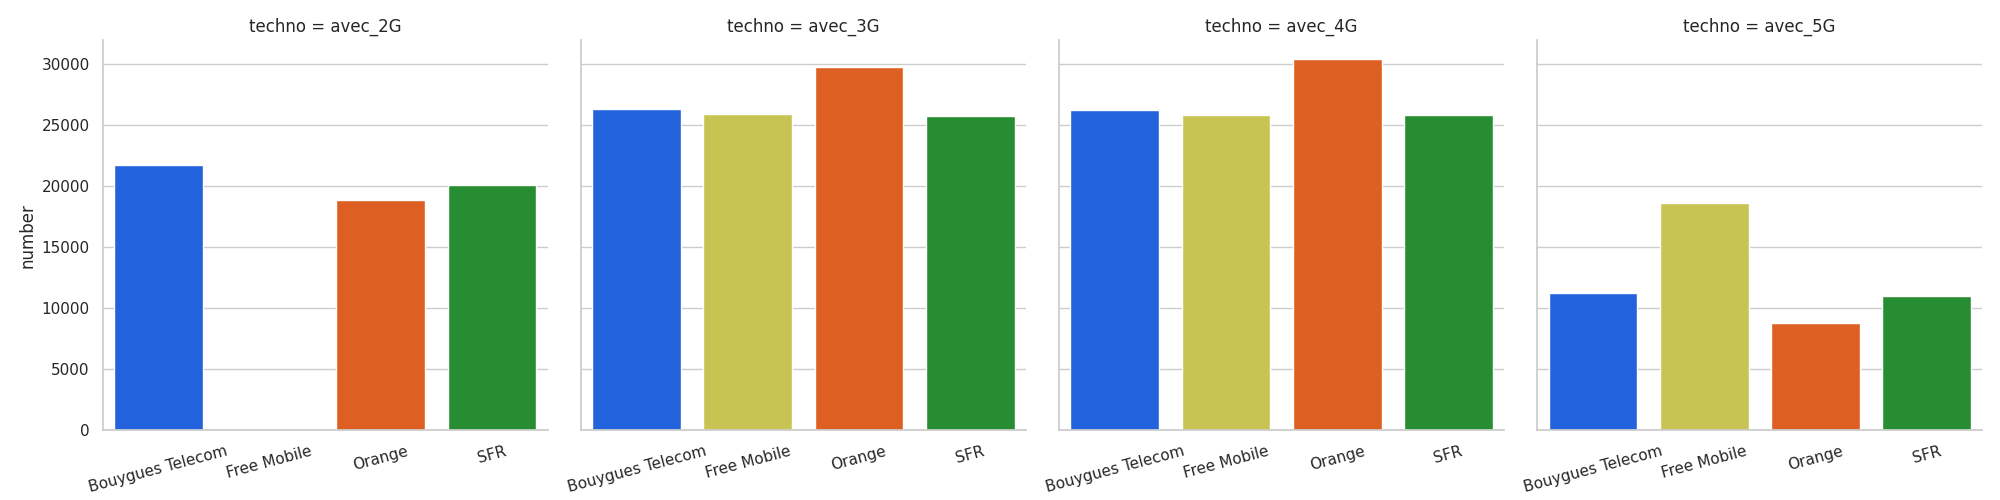
\includegraphics[height=0.4\paperheight]{images/barplots/avec_techno.png}
        \caption{\label{fig:av_tech}Nombres de sites équipés d'au moins une technologie}
    \end{figure}
\end{frame}

\begin{frame}{Comparaison des différents équipements en terme de technologies (2/7)}
    \begin{table}[!ht]
        \centering
        \footnotesize
        \begin{tabular}{cccccc}
        \hline
            \textbf{Technologie} & \textbf{Bouygues Telecom} & \textbf{Free Mobile} & \textbf{Orange} & \textbf{SFR} & \textbf{Total} \\ \hline
            \textbf{2G} & 4 & 0 & 10 & 20 & 34 \\ 
            \textbf{3G} & 30 & 102 & 65 & 37 & 234 \\ 
            \textbf{4G} & 15 & 15 & 602 & 106 & 738 \\ 
            \textbf{5G} & 0 & 0 & 3 & 0 & 3 \\ 
            \textbf{2-3G} & 66 & 0 & 21 & 80 & 167 \\ 
            \textbf{2-4G} & 12 & 0 & 63 & 67 & 142 \\ 
            \textbf{2-5G} & 0 & 0 & 0 & 0 & 0 \\ 
            \textbf{3-4G} & 3889 & 7225 & 9288 & 4909 & 25311 \\ 
            \textbf{3-5G} & 0 & 0 & 0 & 0 & 0 \\ 
            \textbf{4-5G} & 6 & 0 & 109 & 38 & 153 \\ 
            \textbf{2-3-4G} & 11044 & 0 & 11697 & 9831 & 32572 \\ 
            \textbf{2-3-5G} & 0 & 0 & 1 & 0 & 1 \\ 
            \textbf{2-4-5G} & 0 & 0 & 5 & 10 & 15 \\ 
            \textbf{3-4-5G} & 681 & 18607 & 1638 & 835 & 21761 \\ 
            \textbf{2-3-4-5G} & 10584 & 0 & 7038 & 10085 & 27707 \\ 
            \textbf{Total} & 26331 & 25949 & 30540 & 26018 & 108838 \\ \hline
        \end{tabular}
        \caption{Résumé des données de présence de technologie}
    \end{table}
\end{frame}

\begin{frame}{Comparaison des différents équipements en terme de technologies (3/7)}
    Maintenant nous nous intéressons à la fréquence de présence de certaines technologies et pas d'autres :
    \begin{figure}
        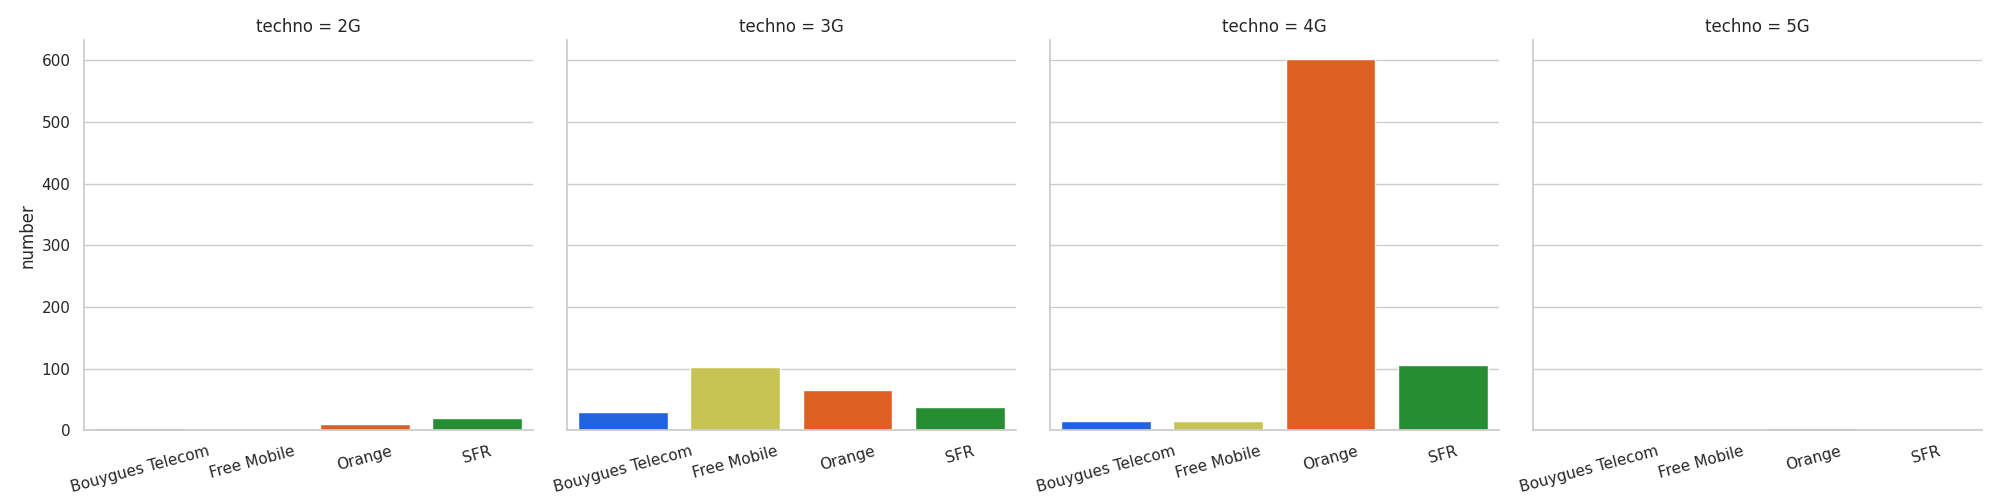
\includegraphics[height=0.4\paperheight]{images/barplots/xG.png}
        \caption{\label{fig:xG}Nombres de sites équipés d'une unique technologie}
    \end{figure}
\end{frame}

\begin{frame}{Comparaison des différents équipements en terme de technologies (4/7)}
    \begin{figure}
        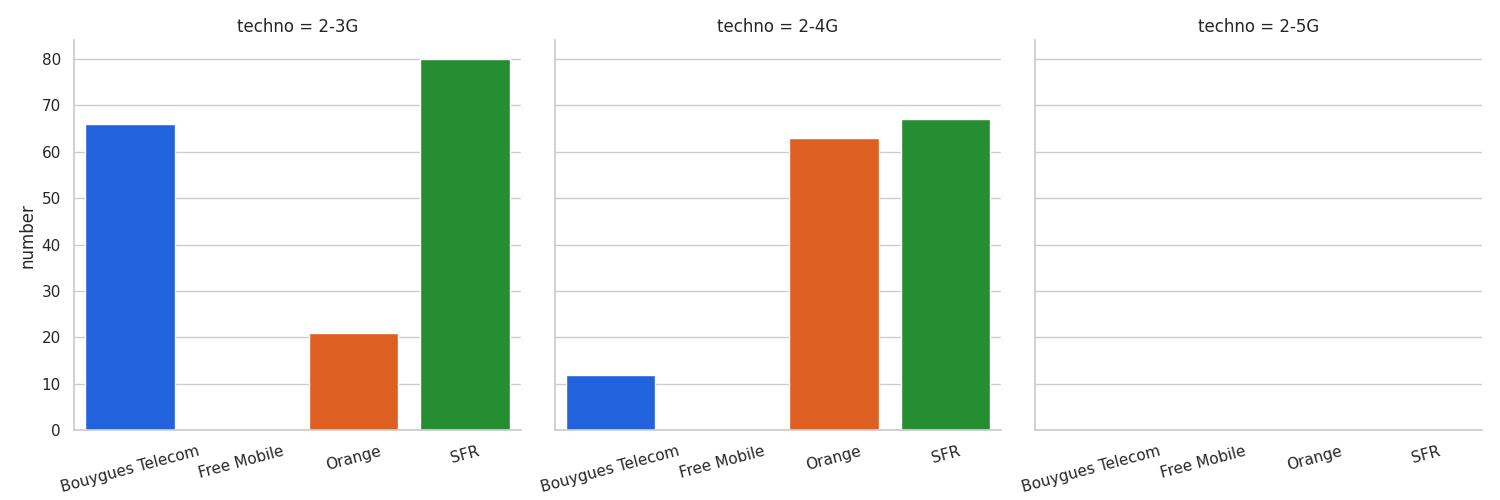
\includegraphics[height=0.4\paperheight]{images/barplots/2-xG.png}
        \caption{\label{fig:2-xG}Nombres de sites équipés de deux technologies}
    \end{figure}
\end{frame}

\begin{frame}{Comparaison des différents équipements en terme de technologies (5/7)}
    \begin{columns}
        \begin{column}{0.65\textwidth}
            \begin{figure}
                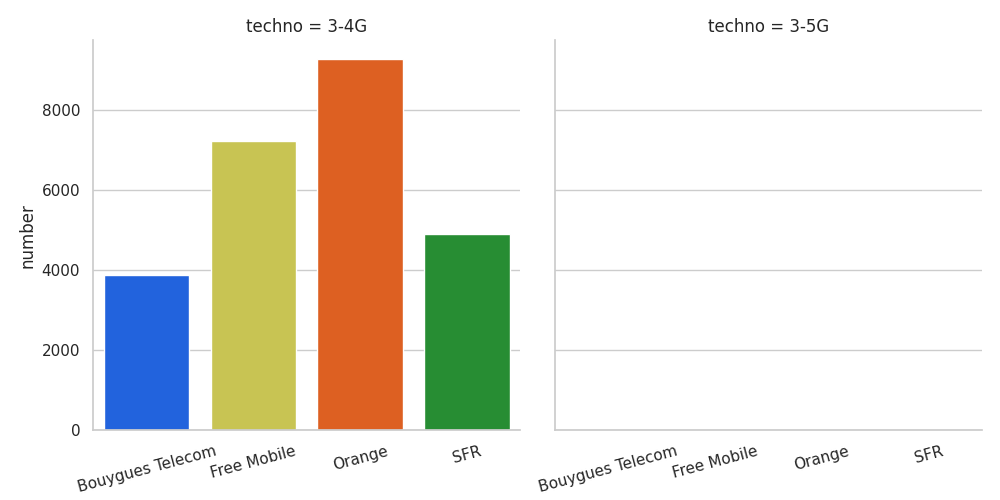
\includegraphics[height=0.4\paperheight]{images/barplots/3-xG.png}
                \caption{\label{fig:3-xG}Nombres de sites équipés de deux technologies (suite)}
            \end{figure}
        \end{column}
            
        \begin{column}{0.35\textwidth}
            \begin{figure}
                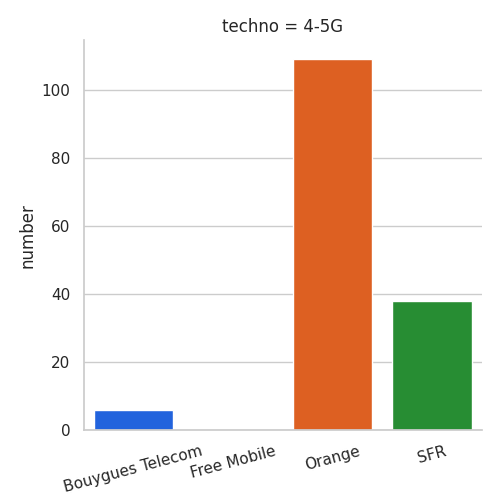
\includegraphics[height=0.4\paperheight]{images/barplots/4-5G.png}
                \caption{\label{fig:4-5G}Nombres de sites équipés de deux technologies (suite-bis)}
            \end{figure}
        \end{column}
    \end{columns} 
\end{frame}

\begin{frame}{Comparaison des différents équipements en terme de technologies (6/7)}
    \begin{figure}
        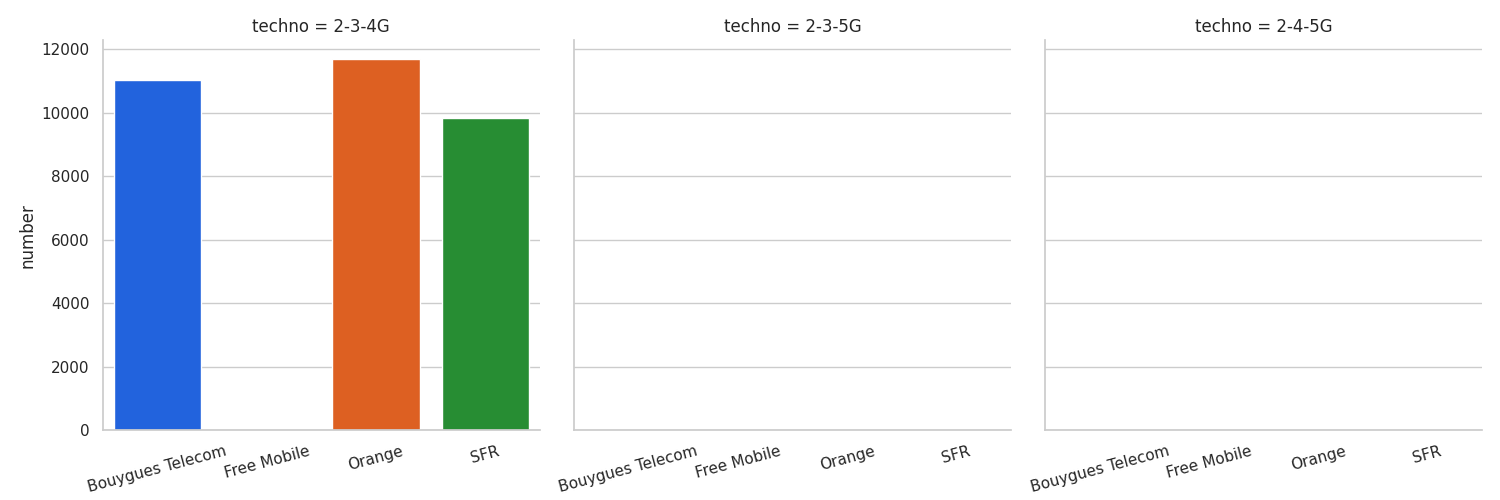
\includegraphics[height=0.4\paperheight]{images/barplots/2-x-yG.png}
        \caption{\label{fig:2-x-yG}Nombres de sites équipés de trois technologies}
    \end{figure}
\end{frame}

\begin{frame}{Comparaison des différents équipements en terme de technologies (7/7)}
    \begin{columns}
        \begin{column}{0.35\textwidth}
            \begin{figure}
                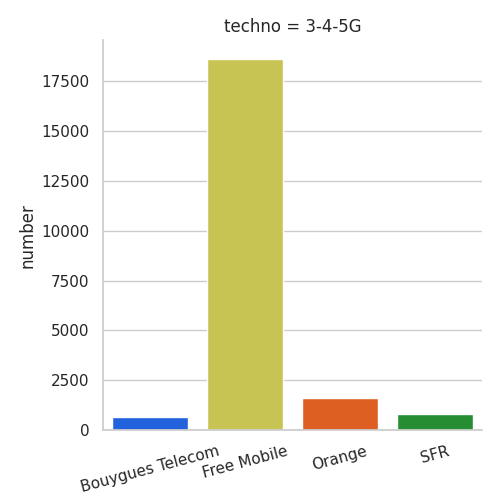
\includegraphics[height=0.4\paperheight]{images/barplots/3-4-5G.png}
                \caption{\label{fig:3-4-5G}Nombres de sites équipés de trois technologies (suite)}
            \end{figure}
        \end{column}
            
        \begin{column}{0.65\textwidth}
            \begin{figure}
                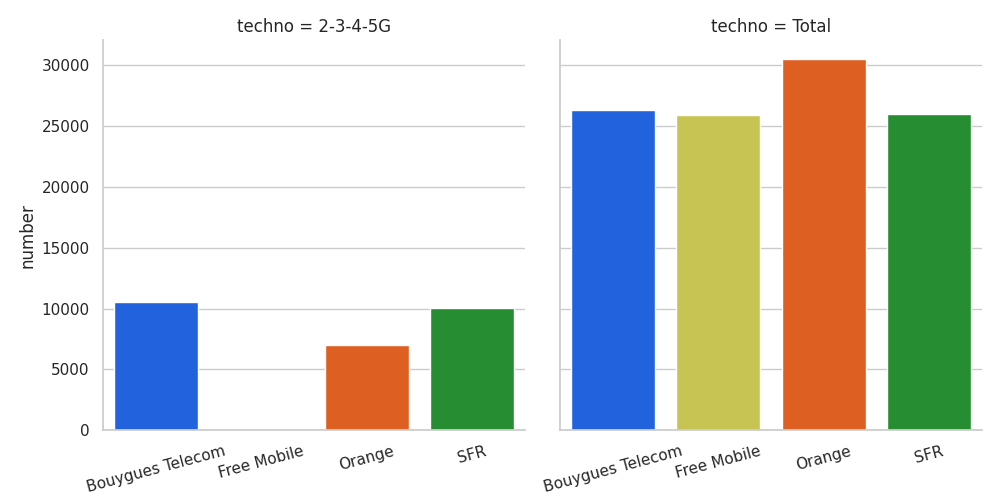
\includegraphics[height=0.4\paperheight]{images/barplots/all-tot.png}
                \caption{\label{fig:all-tot}Nombre de sites équipés de toutes les technologies et total}
            \end{figure}
        \end{column}
    \end{columns} 
\end{frame}

\subsection{Affichage plus détaillé des cartes}
\insertsubsectionframe

\subsubsection{Les stations de base par opérateurs}
\begin{frame}{Les stations de base par opérateur}
    \begin{figure}
        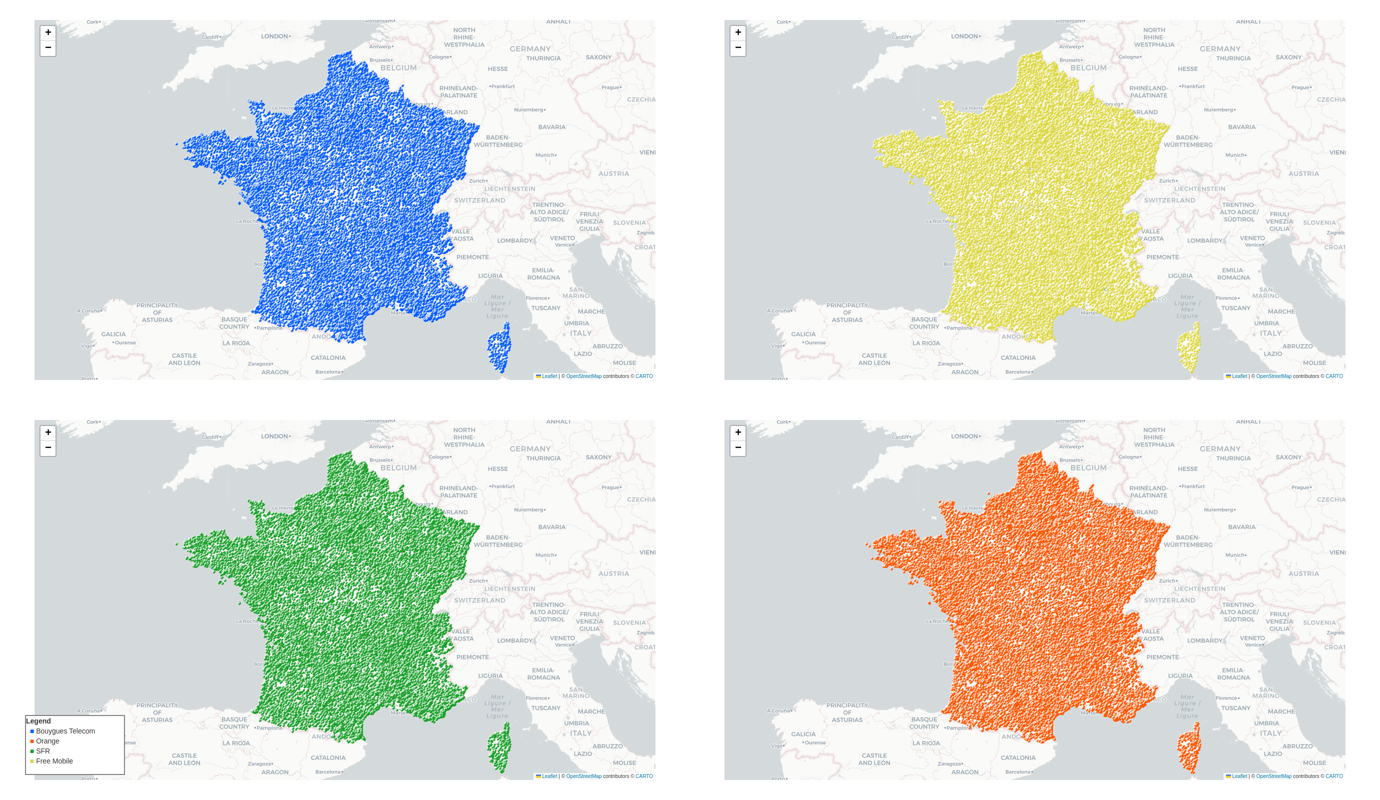
\includegraphics[width=0.9\paperheight]{images/cartes/subplots-providers.png}
        \caption{\label{fig:sp-prov}Les stations de base par opérateurs}
    \end{figure}
\end{frame}


\subsubsection{Les technologies par opérateurs}
\subsubsection{Les technologies par opérateurs}
\begin{frame}{Les stations 2G}
    \begin{figure}
        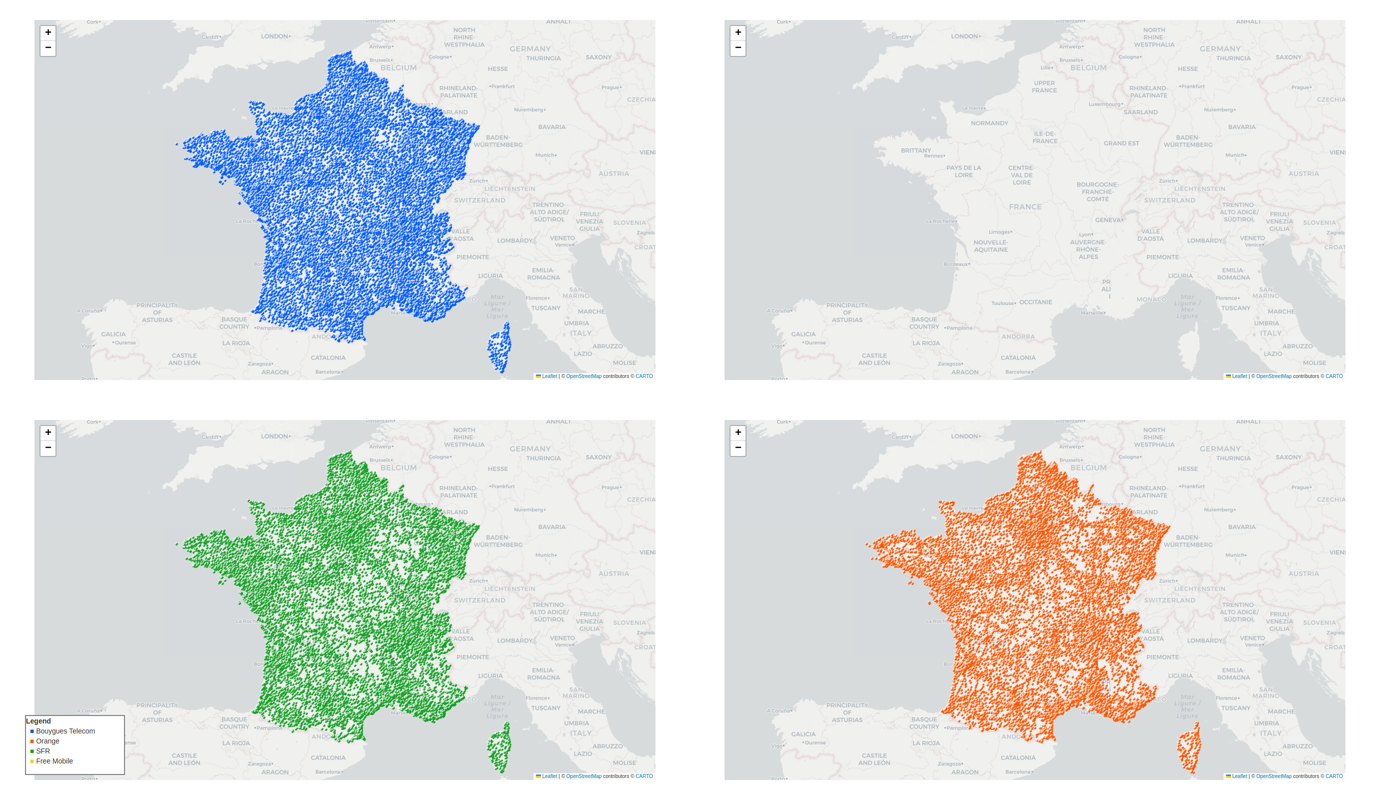
\includegraphics[width=0.9\paperheight]{images/cartes/providers-site_2g.png}
        \caption{\label{fig:sp-2g}Les stations 2G}
    \end{figure}
\end{frame}

\begin{frame}{Les stations 3G}
    \begin{figure}
        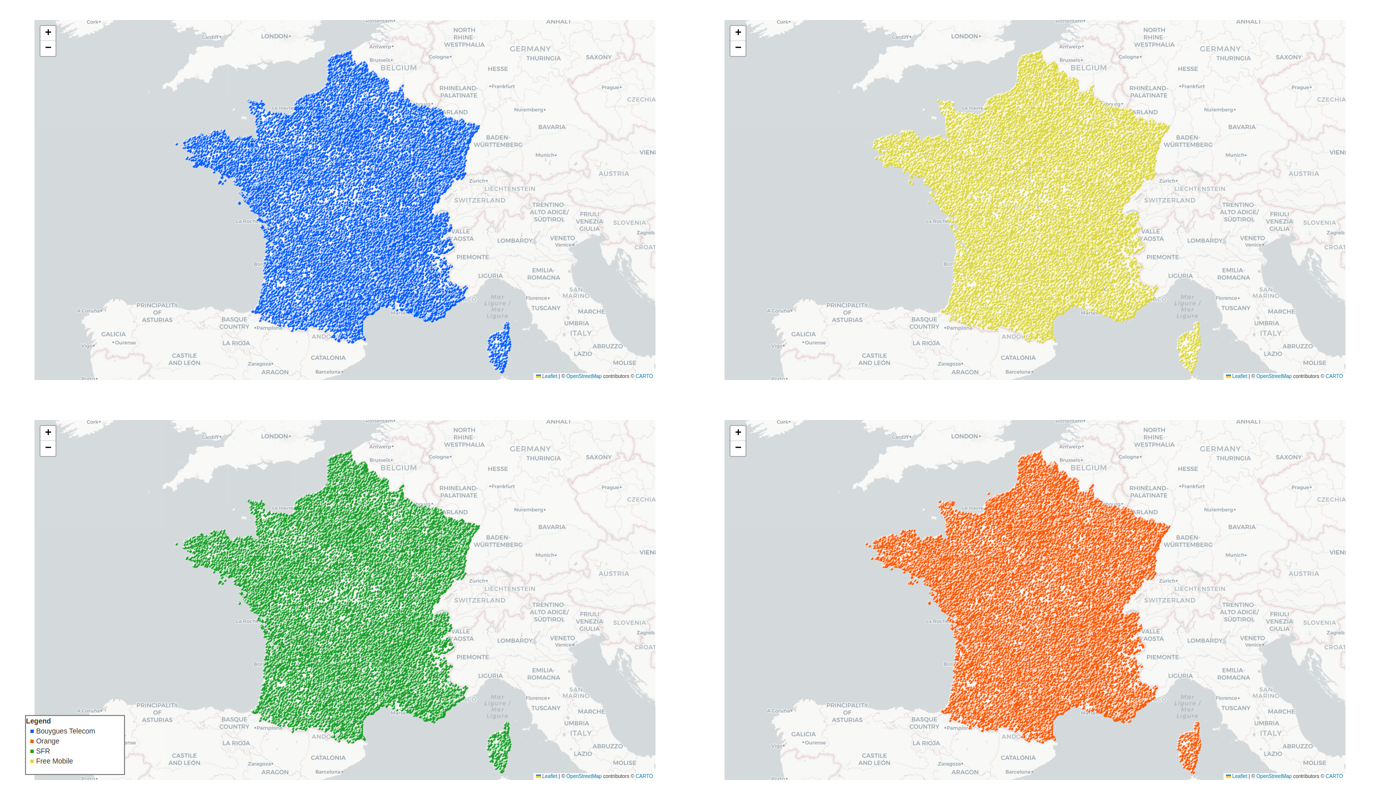
\includegraphics[width=0.9\paperheight]{images/cartes/providers-site_3g.png}
        \caption{\label{fig:sp-3g}Les stations 3G}
    \end{figure}
\end{frame}

\begin{frame}{Les stations 4G}
    \begin{figure}
        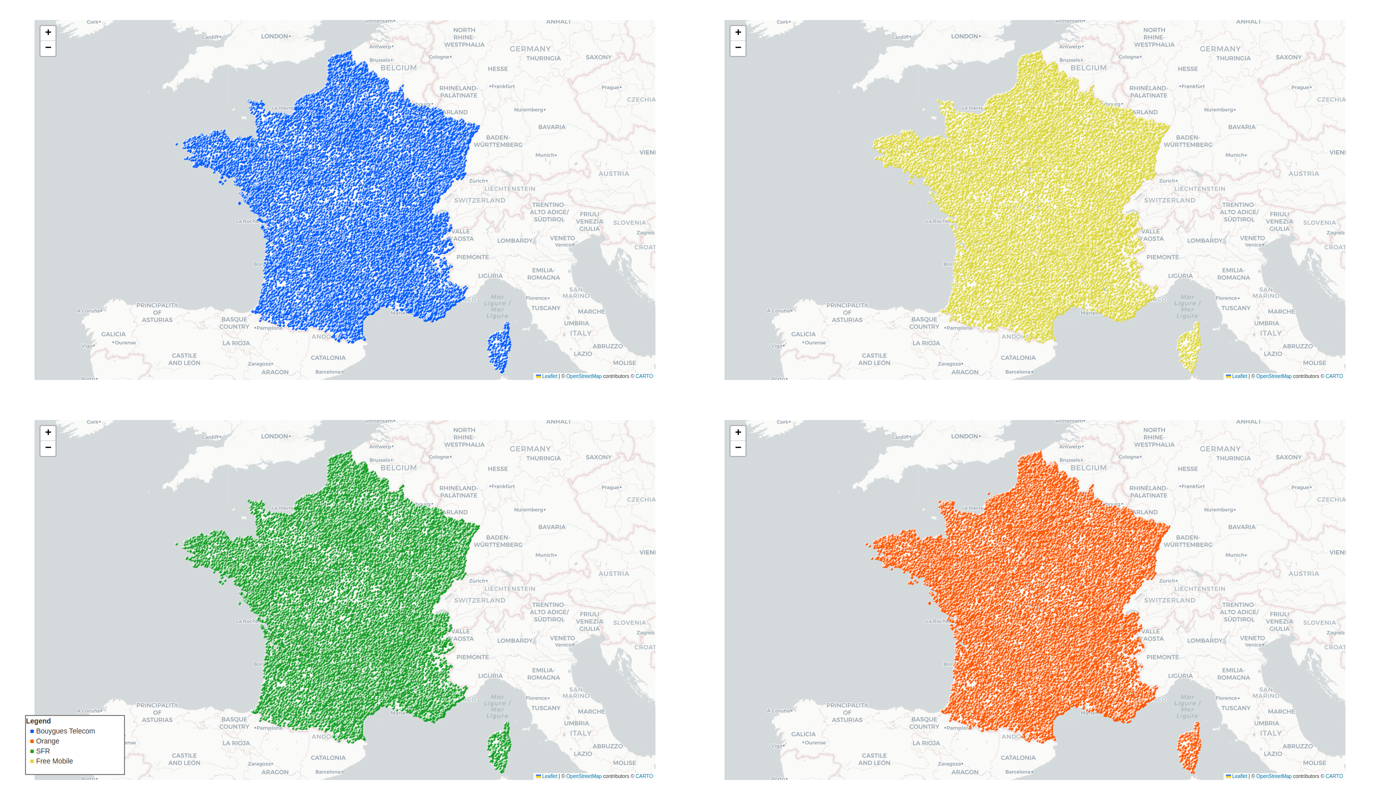
\includegraphics[width=0.9\paperheight]{images/cartes/providers-site_4g.png}
        \caption{\label{fig:sp-4g}Les stations 4G}
    \end{figure}
\end{frame}

\begin{frame}{Les stations 5G}
    \begin{figure}
        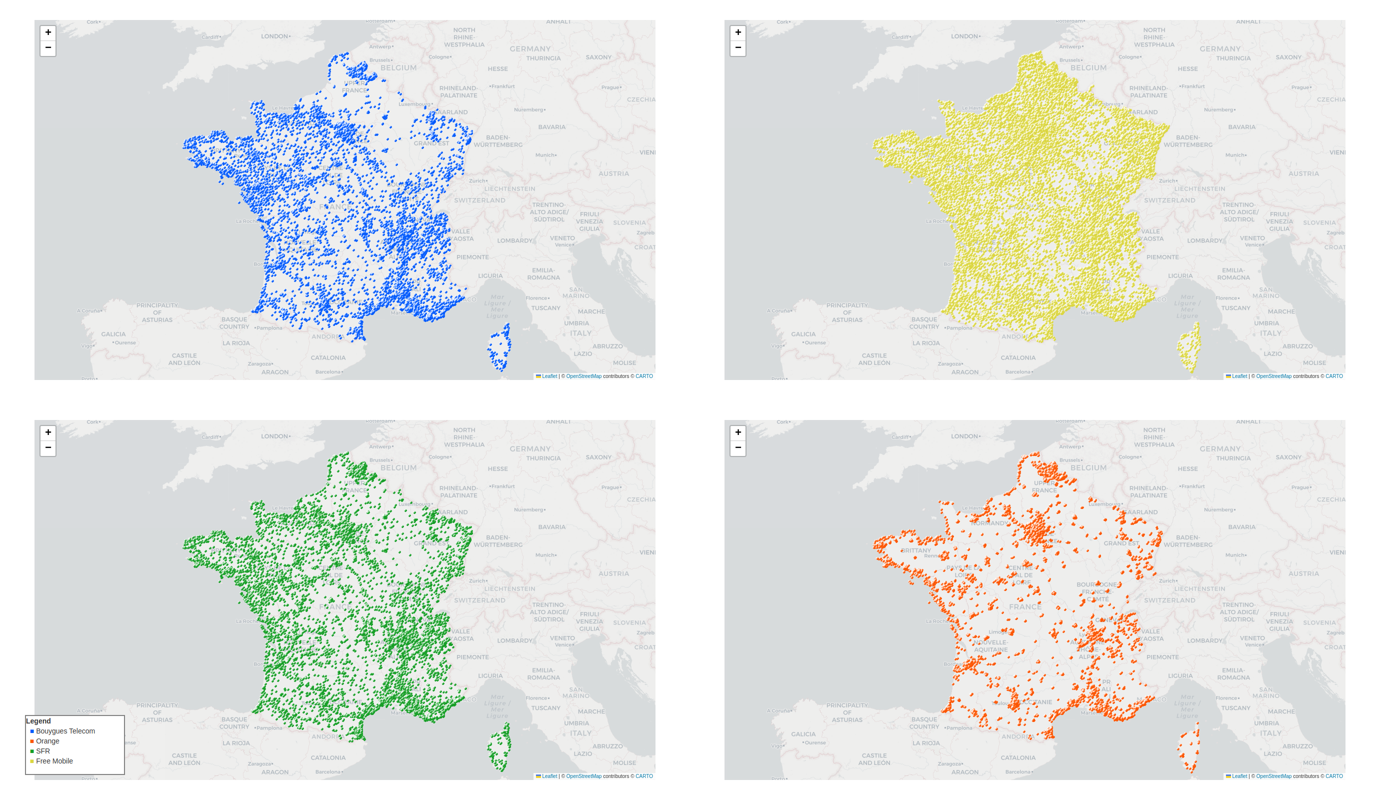
\includegraphics[width=0.9\paperheight]{images/cartes/providers-site_5g.png}
        \caption{\label{fig:sp-5g}Les stations 5G}
    \end{figure}
\end{frame}


\subsection{Evolution du nombre de stations de base au cours du temps}
\insertsubsectionframe

\begin{frame}{2023\_T4\_sites\_5G\_historique\_comptage}
    \begin{figure}
        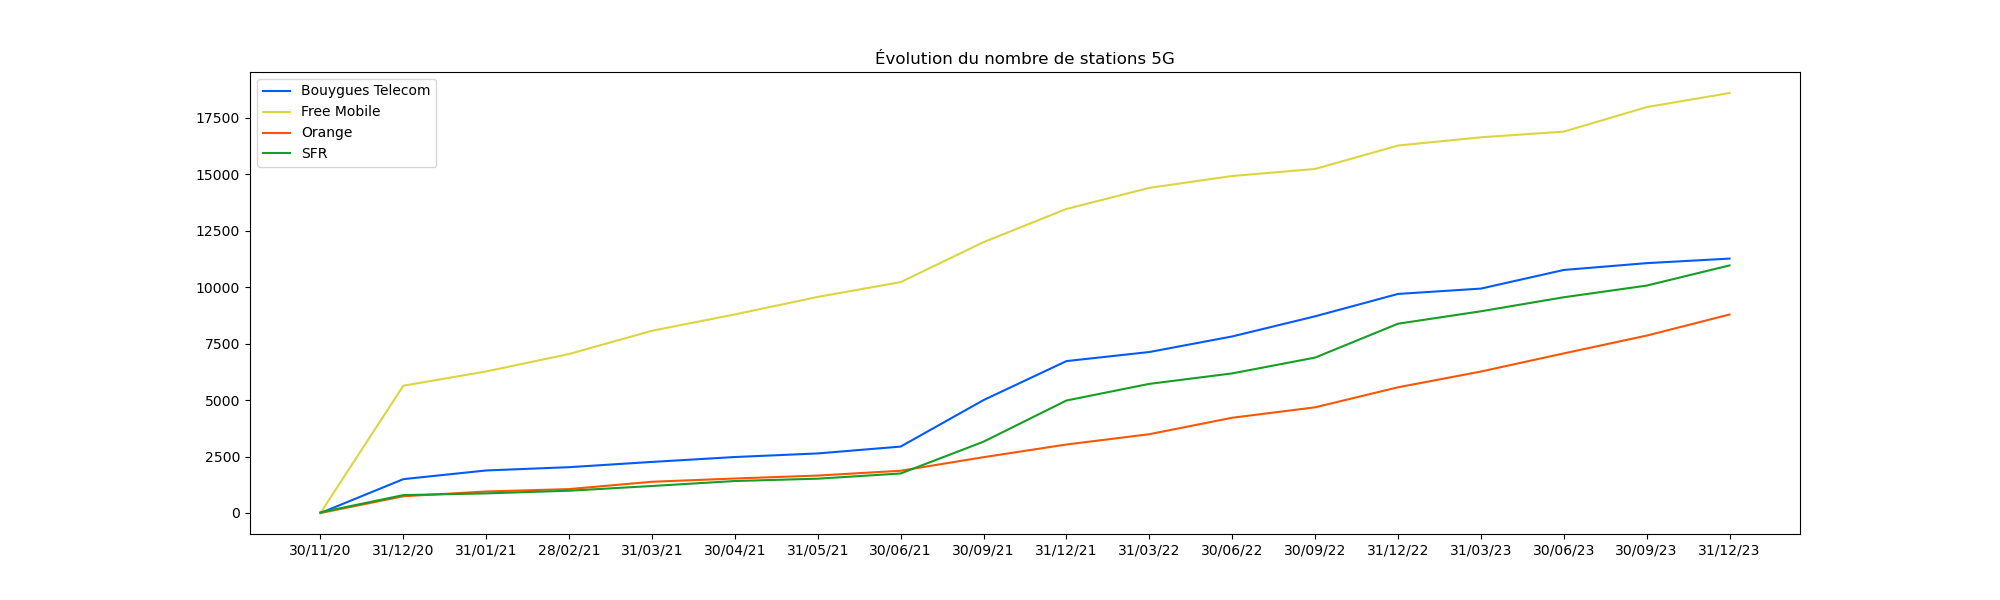
\includegraphics[height=0.5\paperheight]{images/5G-evolution.png}
        \caption{\label{fig:5G-ev}Evolution du nombre de stations 5G en France}
    \end{figure}
\end{frame}


\begin{frame}{Compilation des jeux de données sites}
    \begin{figure}
        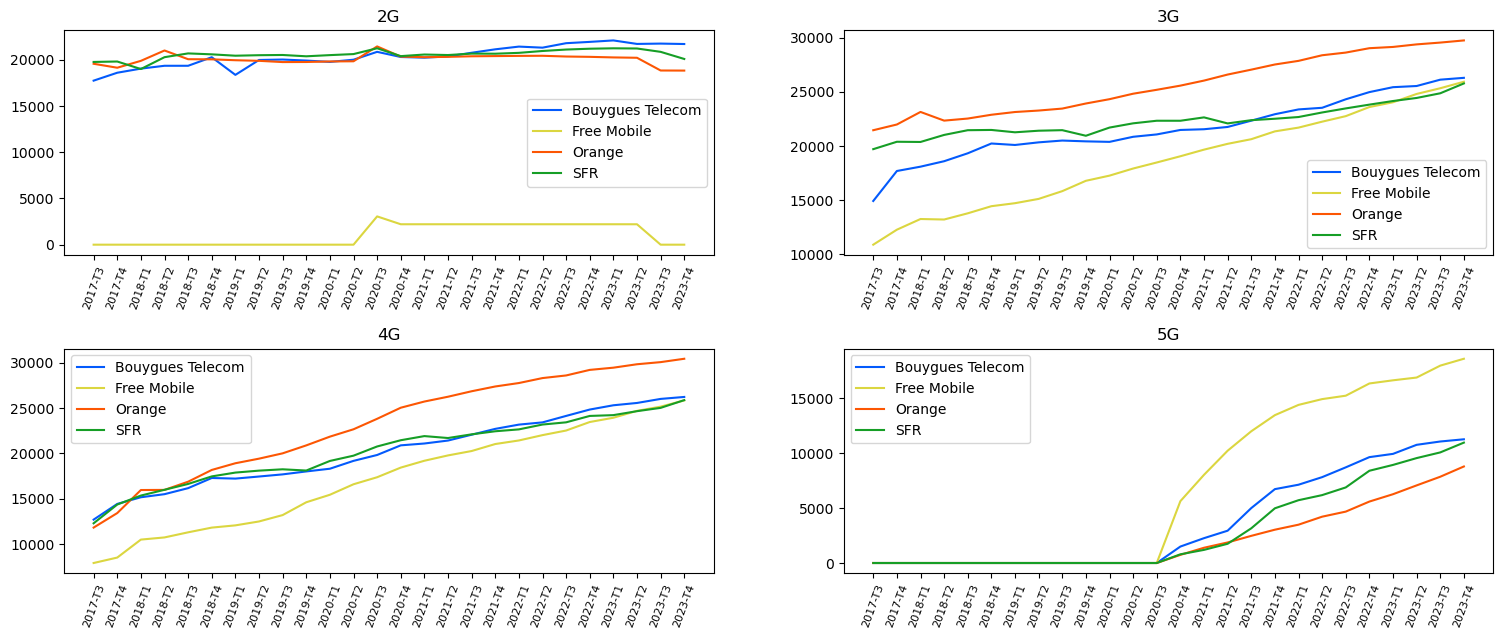
\includegraphics[width=0.78\paperwidth]{images/technos-evolution.png}
        \caption{\label{fig:techno-ev} Evolution du nombre de stations toutes technologies en France}
    \end{figure}
\end{frame}

\begin{frame}{Dispositif de couverture ciblée, éléments d'analyse}
    \begin{block}{infos générales}
        \begin{itemize}
            \item 4621 stations de bases potentielles;
            \item 26 attributs.
        \end{itemize}
    \end{block}

    \begin{block}{anomalies}
        \begin{itemize}
            \item 412 lignes de ce jeu de données ont les colonnes \textbf{x\_lambert\_93} ou \textbf{y\_lambert\_93} non renseigné;
            \item Plusieurs points sont placés en dehors de la France.
        \end{itemize}
    \end{block}
\end{frame}


\begin{frame}{Dispositif de couverture ciblée}
    \begin{figure}
        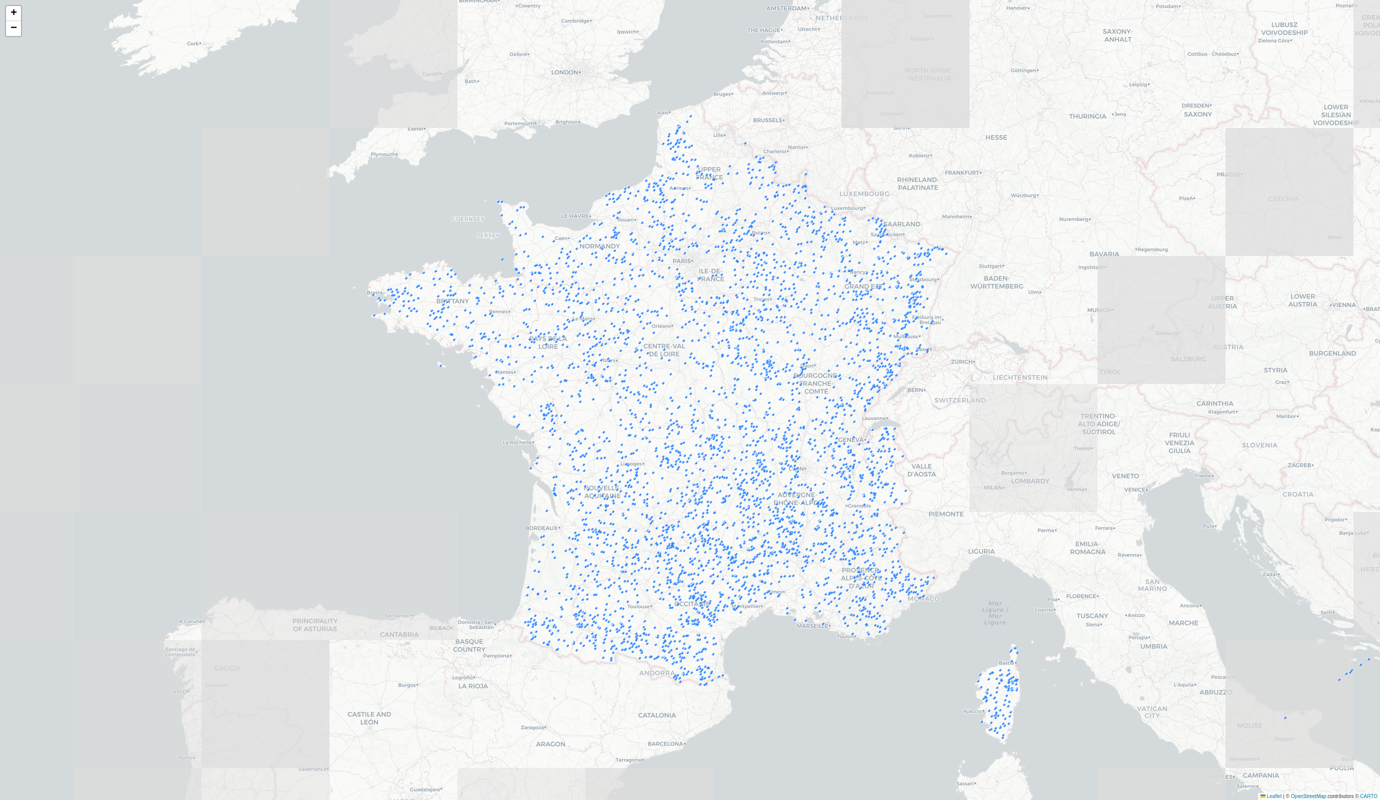
\includegraphics[height=.8\textheight]{images/couverture_ciblee.png}
    \end{figure}
\end{frame}

\begin{frame}{Couverture théorique}
    \begin{block}{Informations}
        \begin{itemize}
            \item format .gpkg (geopackage)
            \item ouverture à l'aide du logiciel libre QGIS
        \end{itemize}
    \end{block}

    \begin{block}{Utilité}
        \begin{itemize}
            \item Aurait pu permettre de déterminer si 2 stations de base sont voisines (si leur couverture se chevauche)
            \item Non réalisable à l'aide de ce jeu de donnée : seule la courverture globale de chaque région est donnée
        \end{itemize}
    \end{block}
\end{frame}

\begin{frame}{}
    \begin{figure}
        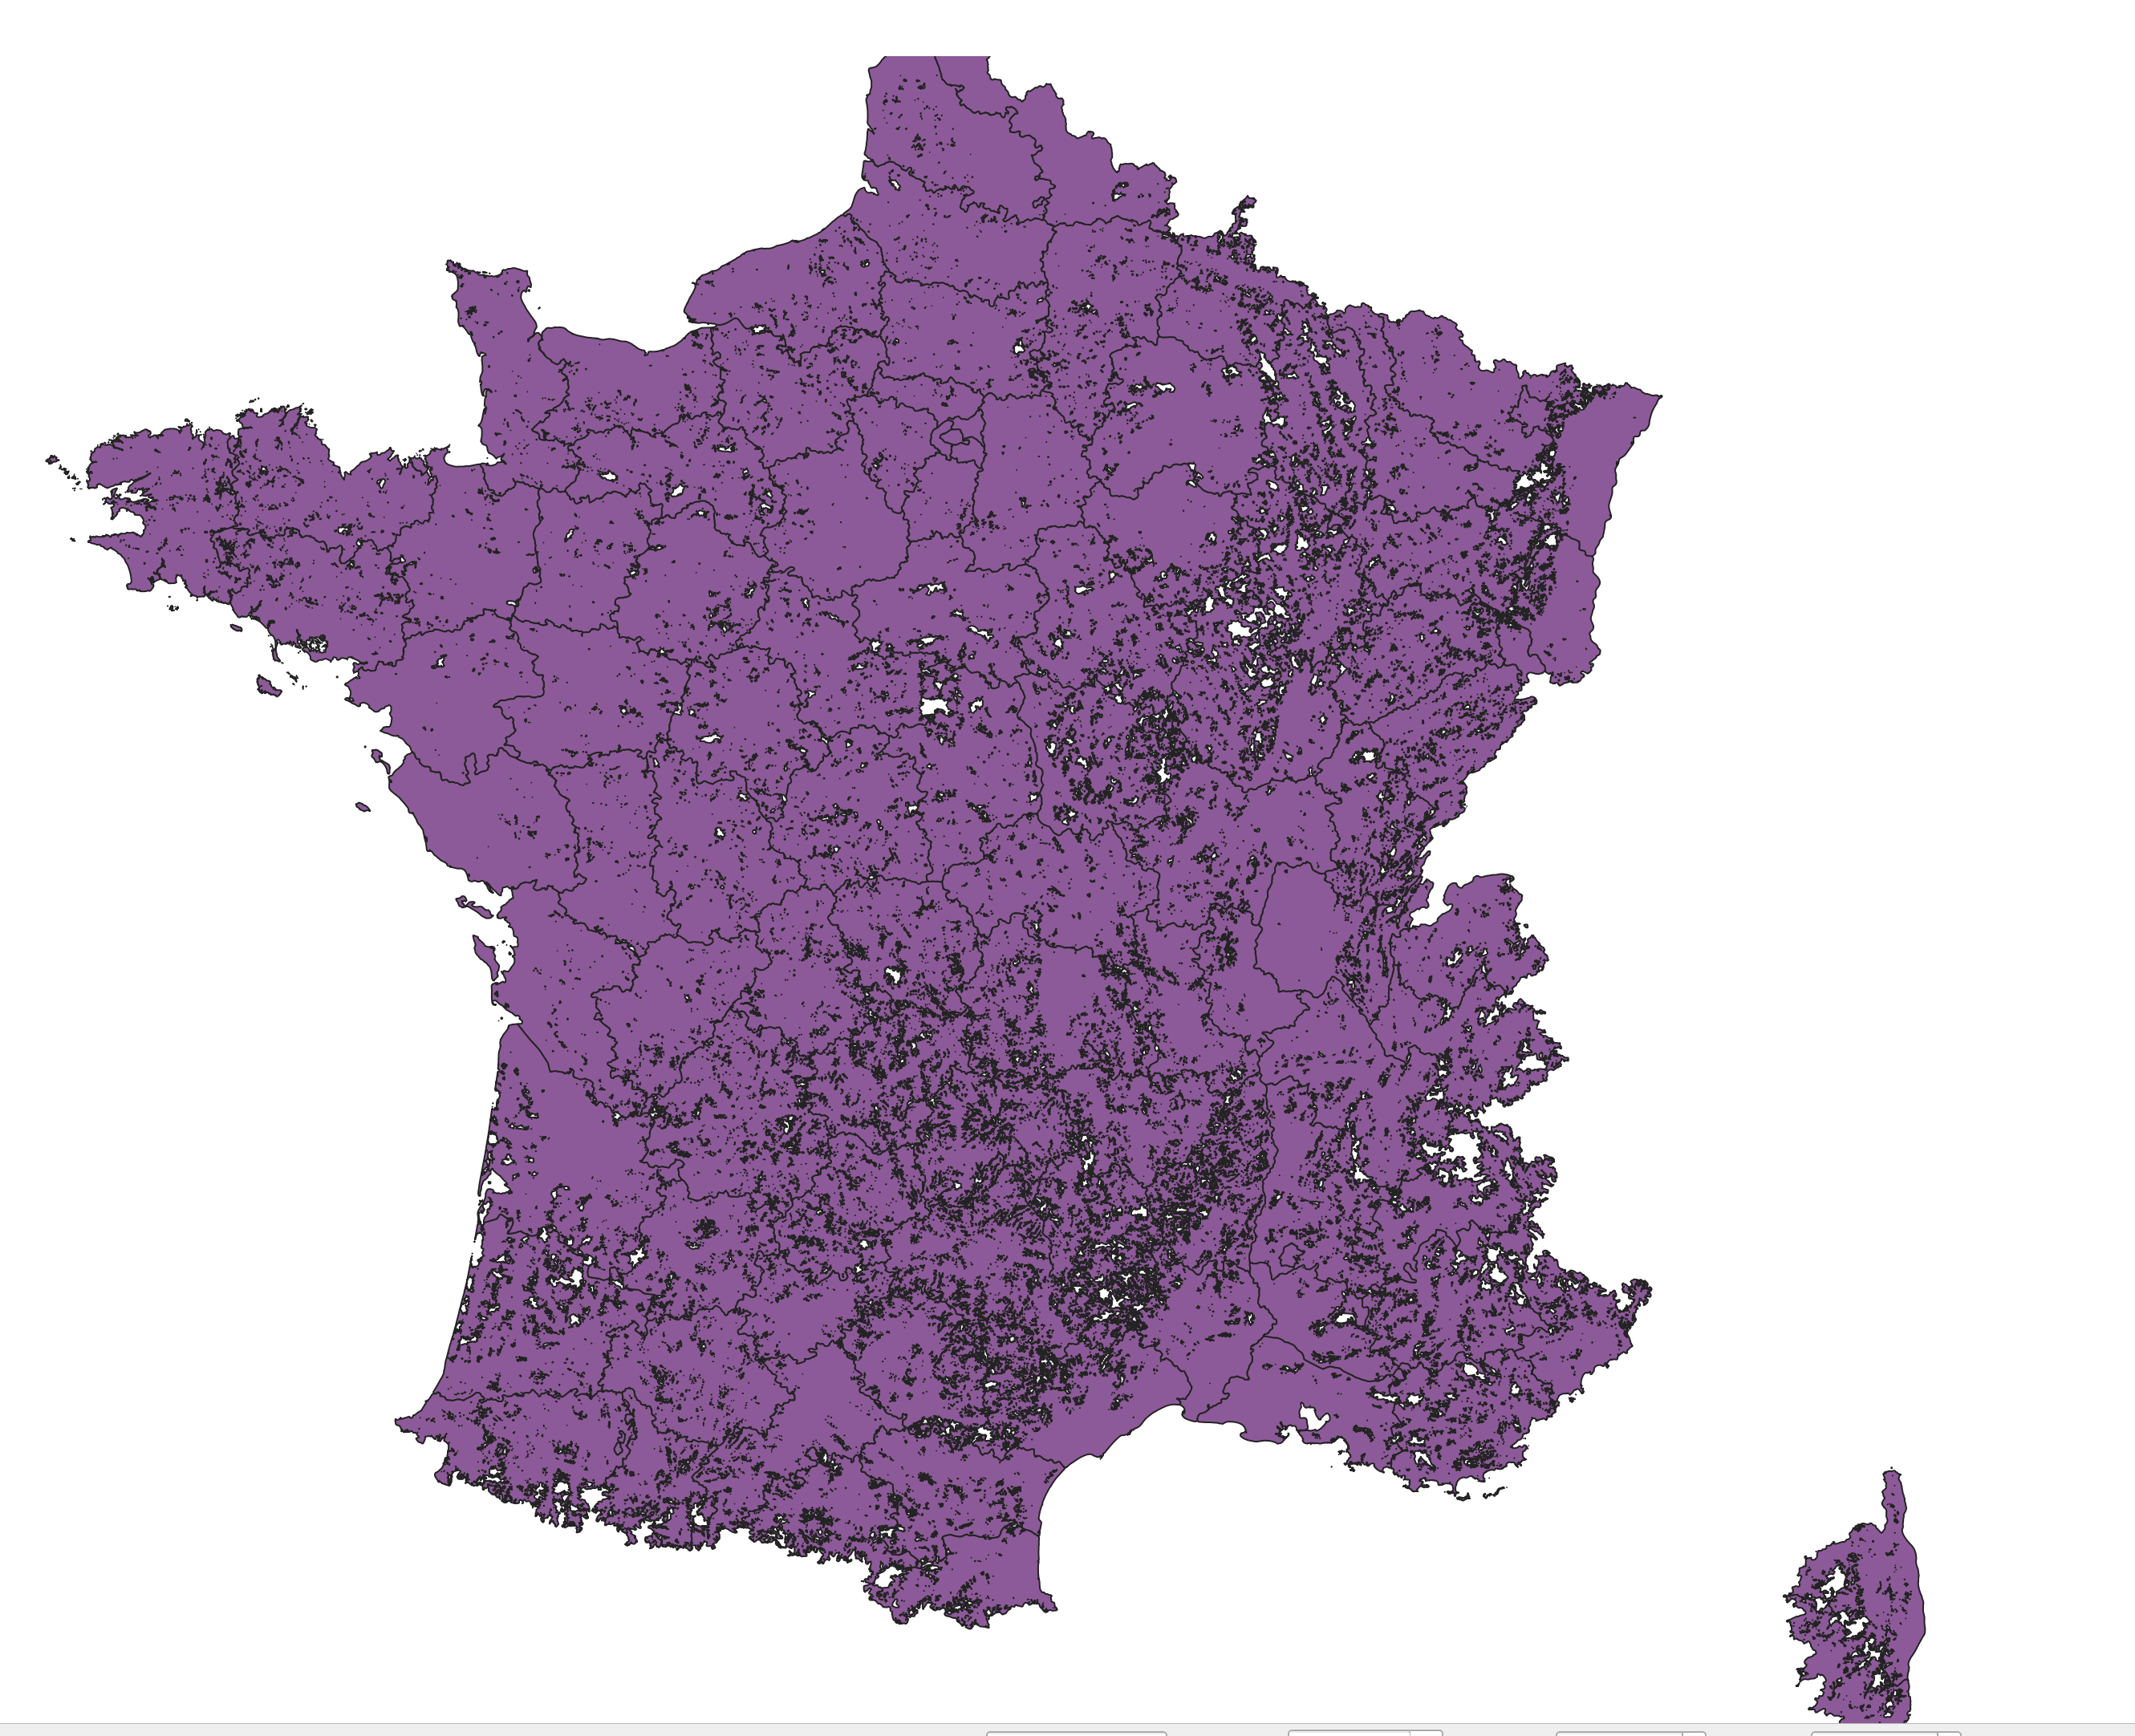
\includegraphics[height=.8\textheight]{images/couverture_theorique_bouygues.png}
    \end{figure}
\end{frame}